\documentclass{article}
\usepackage{graphicx} % Required for inserting images
\usepackage{amsmath} 
\usepackage{float}
\usepackage{listings}

\newcommand{\probP}{\text{I\kern-0.15em P}}
\newcommand {\sig}{(1 + e^{-\theta^Tx_{i}})}

\title{Assignment-4}
\author{Surendra Parla}
\date{4 March 2024}

\begin{document}

\maketitle

\section{1}
Instead of binary normalization I have used quantiles which are customizable through the parameter "num\_of\_splits\_per\_feature". For example if we choose this hyper parameter as 3 we would validate 25 percentile, 50 percentile (median) and 75 percentile and take the best of these (which gives maximum mutual information).
\section{2}
Mutual Information $I(x_j, y)$ is calculted by the function "mutual\_information" (code in the appendix).
\section{3}
Generalized Decision Tree is implemented as the code is provided in the appendix.
The stopping criteria used in this code is either small mutual information of about 0.05 is reached or when the subsample size is less than or equal to 5 percent of entire dataset. These, fields can be adjusted through parameters and can be tuned as hyper parameters as well to avoid overfitting.
\section{4}
Decision Tree obtained from the dataset is:
\begin{figure}
    \ffigbox{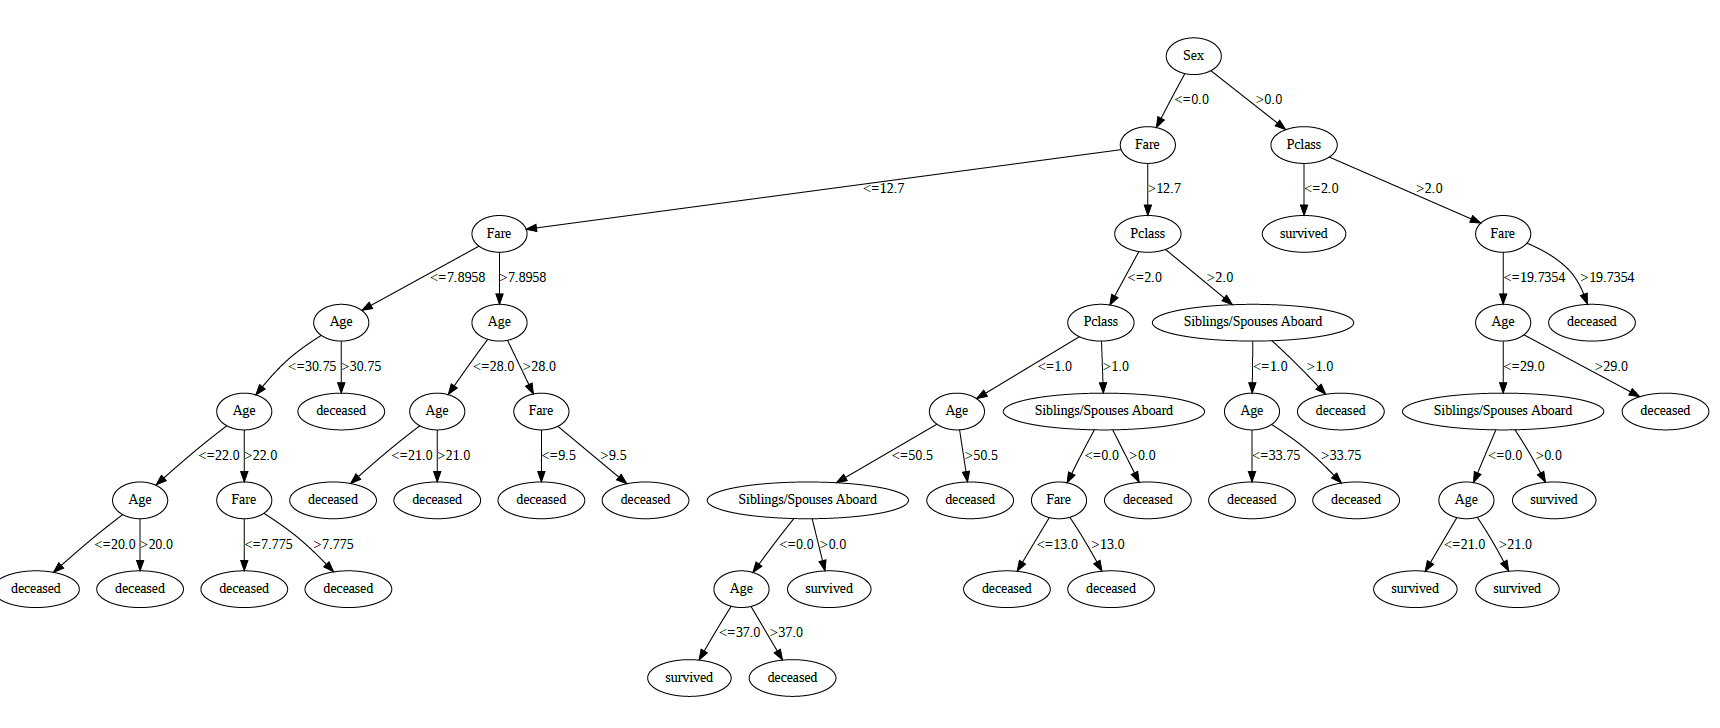
\includegraphics[width=1\textwidth]{decision-tree/dt.png}}
    \caption{Decision Tree for Titanic Dataset}
\end{figure}
\section{5}
Code for cross validation is attached in the appendix and the accuracy is 79.54
\section{6}
My feature vector is \\
X = 
$
\begin{pmatrix}
    2 \\
    0 \\
    25 \\
    0 \\
    0 \\
    20
\end{pmatrix} \\
$
The out from decision tree is 0 which represents I would be deceased which is inline with what we observed in logistic regression.

\section{7}
\subsection{a}
Random forest for 80\% random data sampling Figure 2 to 6
\begin{center}
\begin{figure}
    \ffigbox{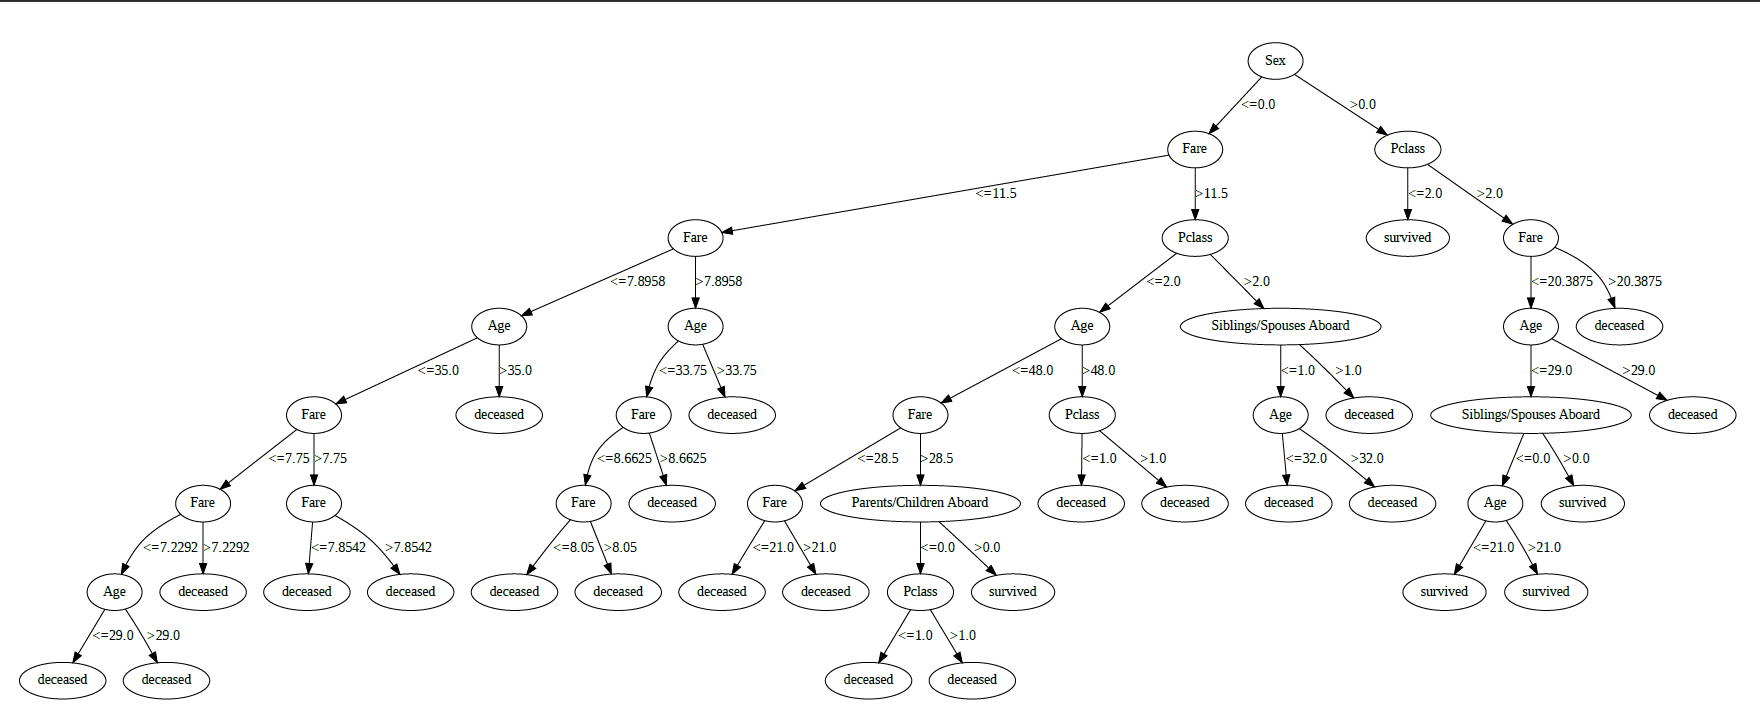
\includegraphics[width=1\textwidth]{random-forest/rf1.png}}
    \caption{Random Forest 1}
\end{figure}
\begin{figure}
    \ffigbox{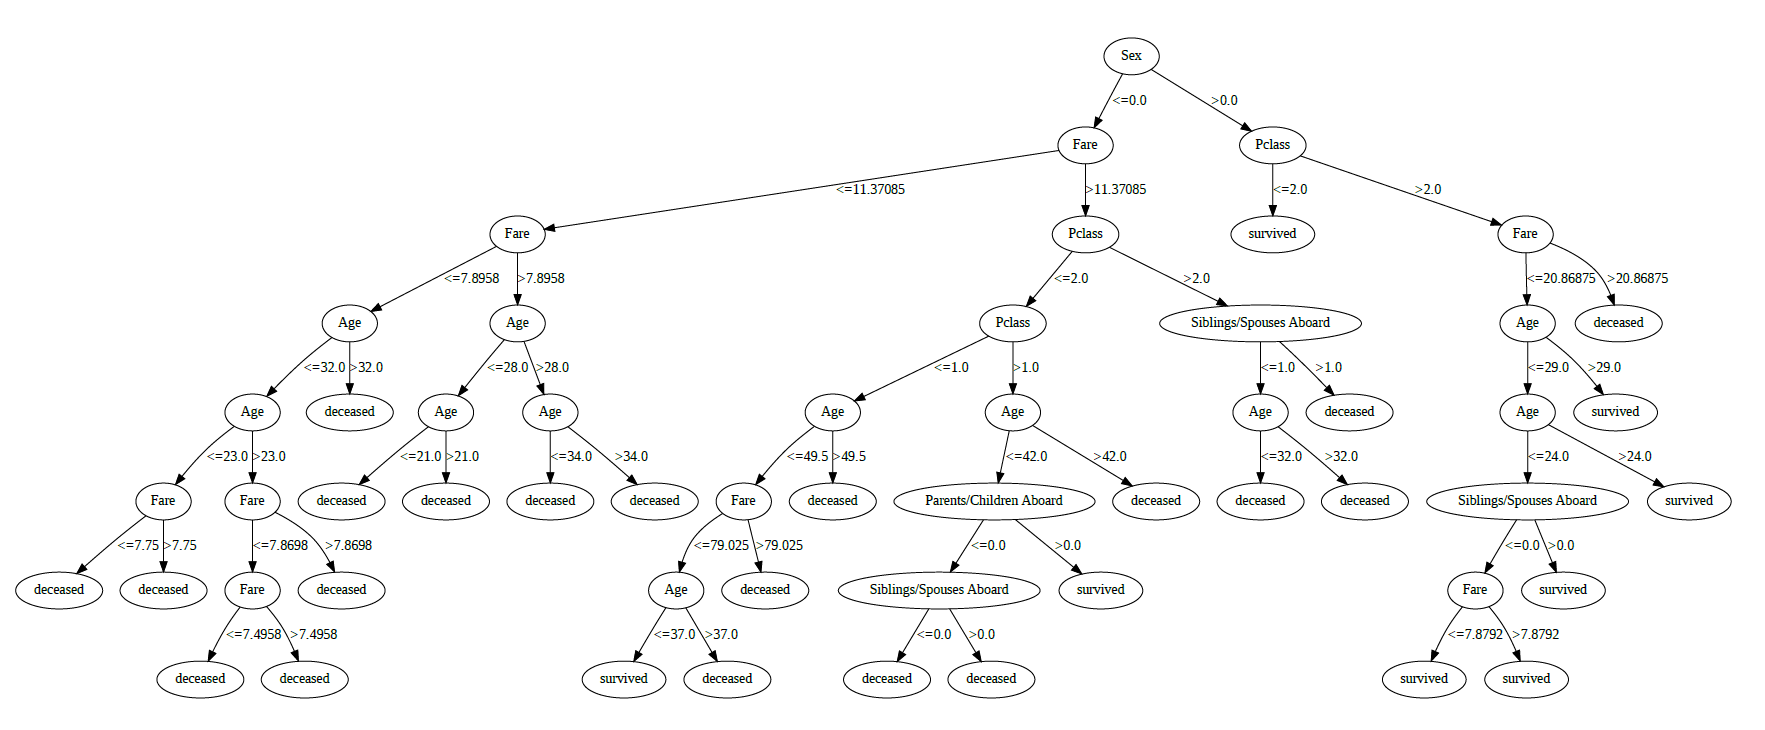
\includegraphics[width=1\textwidth]{random-forest/rf2.png}}
    \caption{Random Forest 2}
\end{figure}
\begin{figure}
    \ffigbox{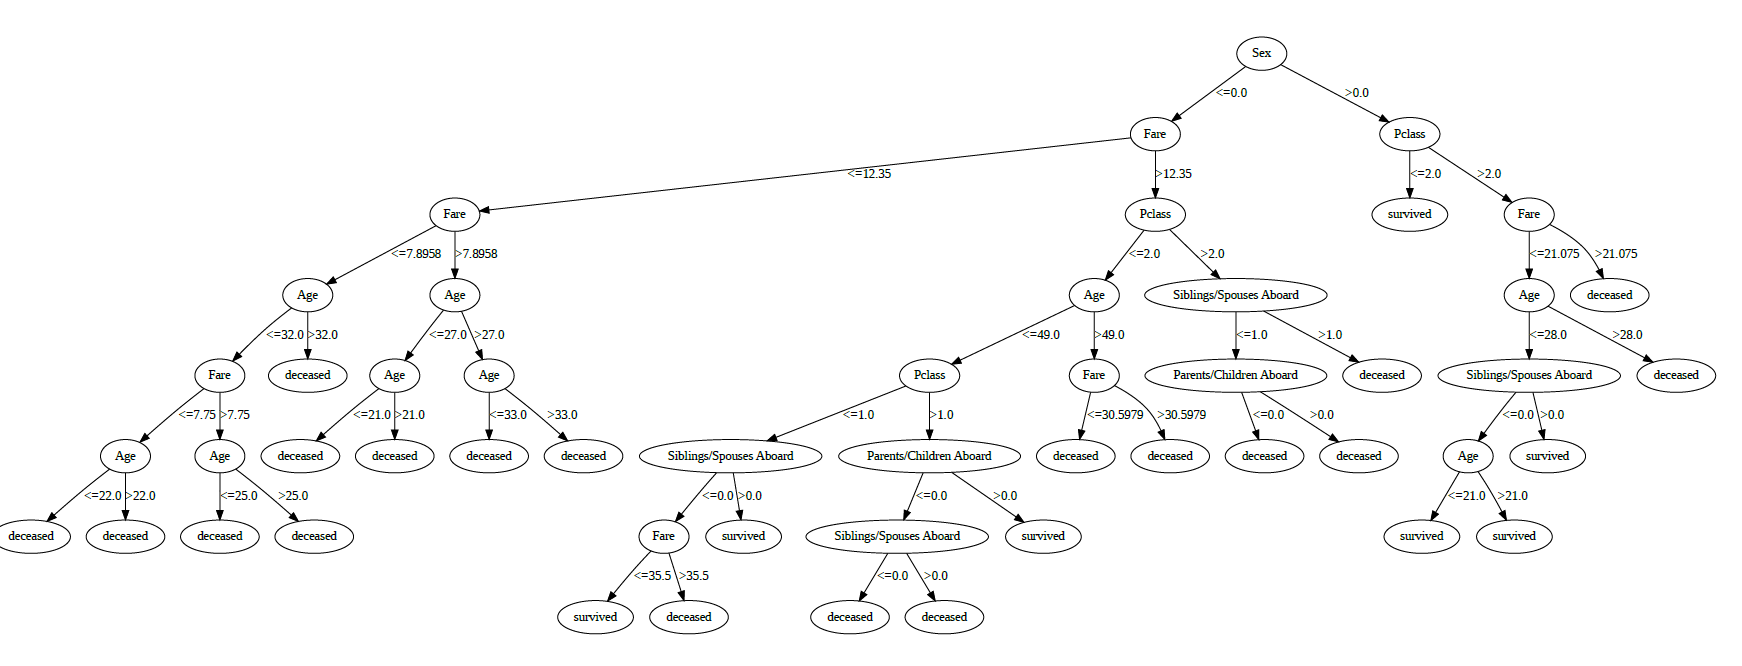
\includegraphics[width=1\textwidth]{random-forest/rf3.png}}
    \caption{Random Forest 3}
\end{figure}
\begin{figure}
    \ffigbox{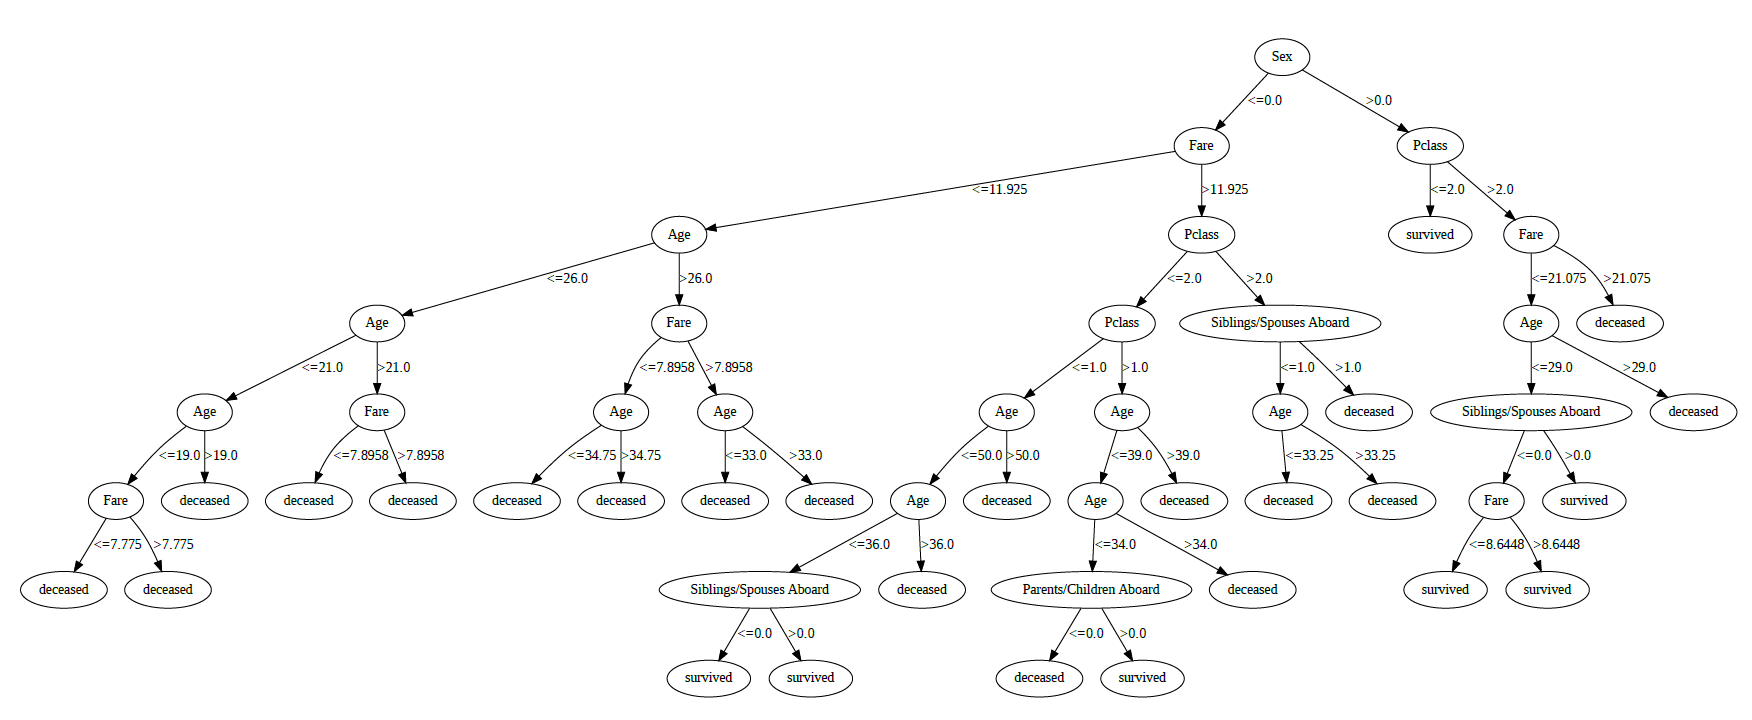
\includegraphics[width=1\textwidth]{random-forest/rf4.png}}
    \caption{Random Forest 4}
\end{figure}
\begin{figure}
    \ffigbox{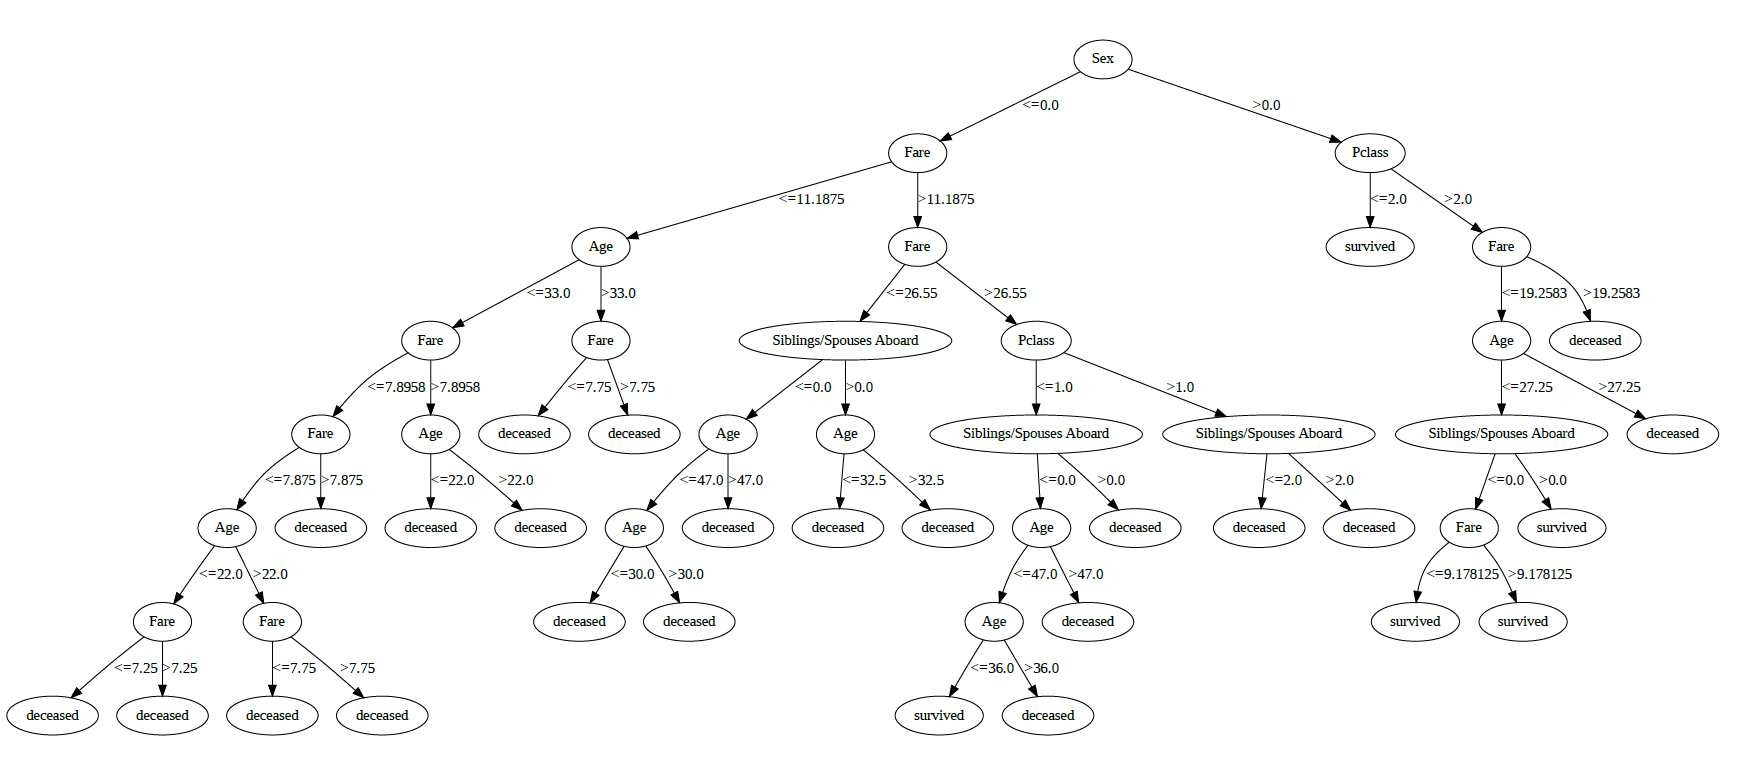
\includegraphics[width=1\textwidth]{random-forest/rf5.png}}
    \caption{Random Forest 5}
\end{figure}
\end{center}
\subsection{b}
Accuracy obtained by 10 fold cross validation on random forest is 79.1\%
\subsection{c}
According to this random forest i would have not survived as all 5 trees predicted 0.

\section{8}
\subsection{a}
Random forest trees: Figure 7 to 12
\begin{figure}
    \ffigbox{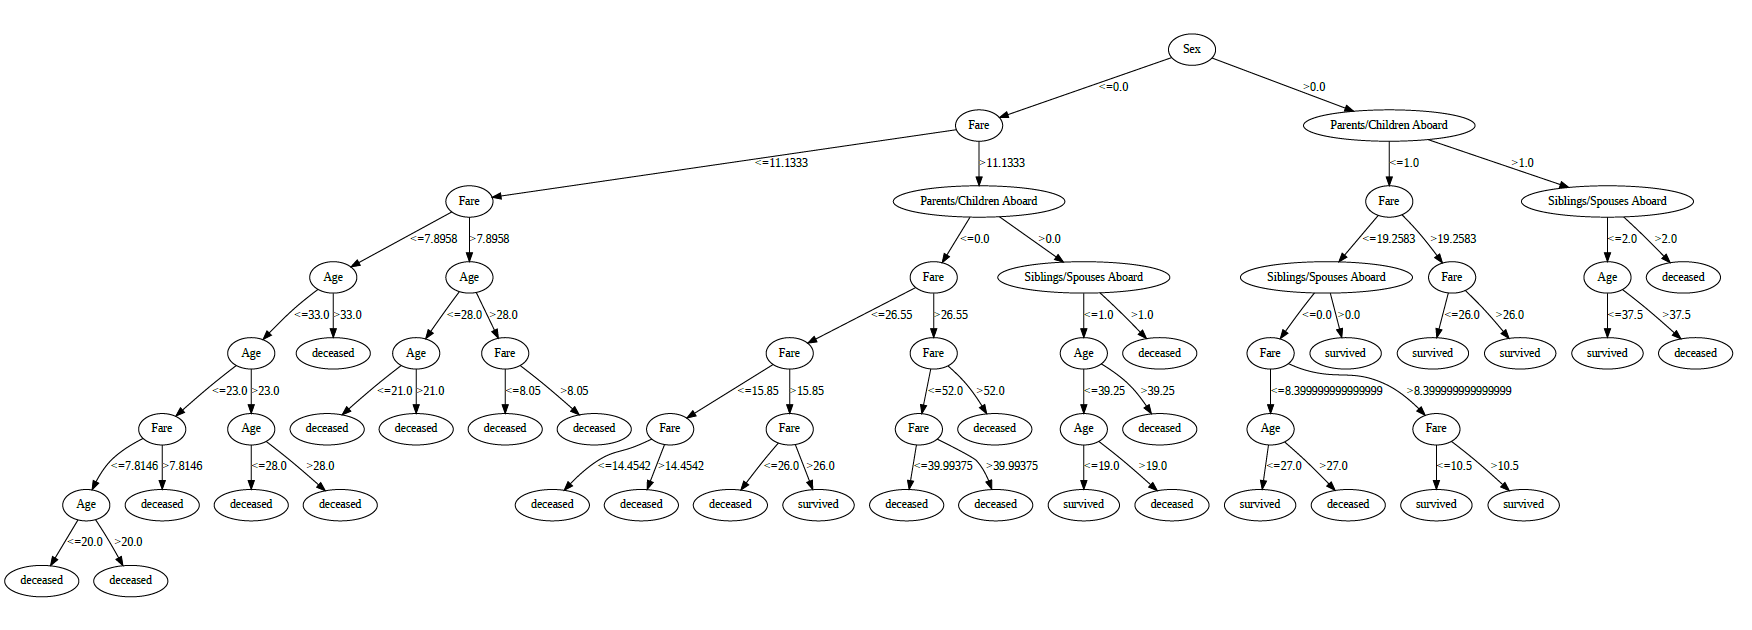
\includegraphics[width=1\textwidth]{rf-feature-dropout/rf_leave_out1.png}}
    \caption{Random Forest excluding feature Pclass}
\end{figure}
\begin{figure}
    \ffigbox{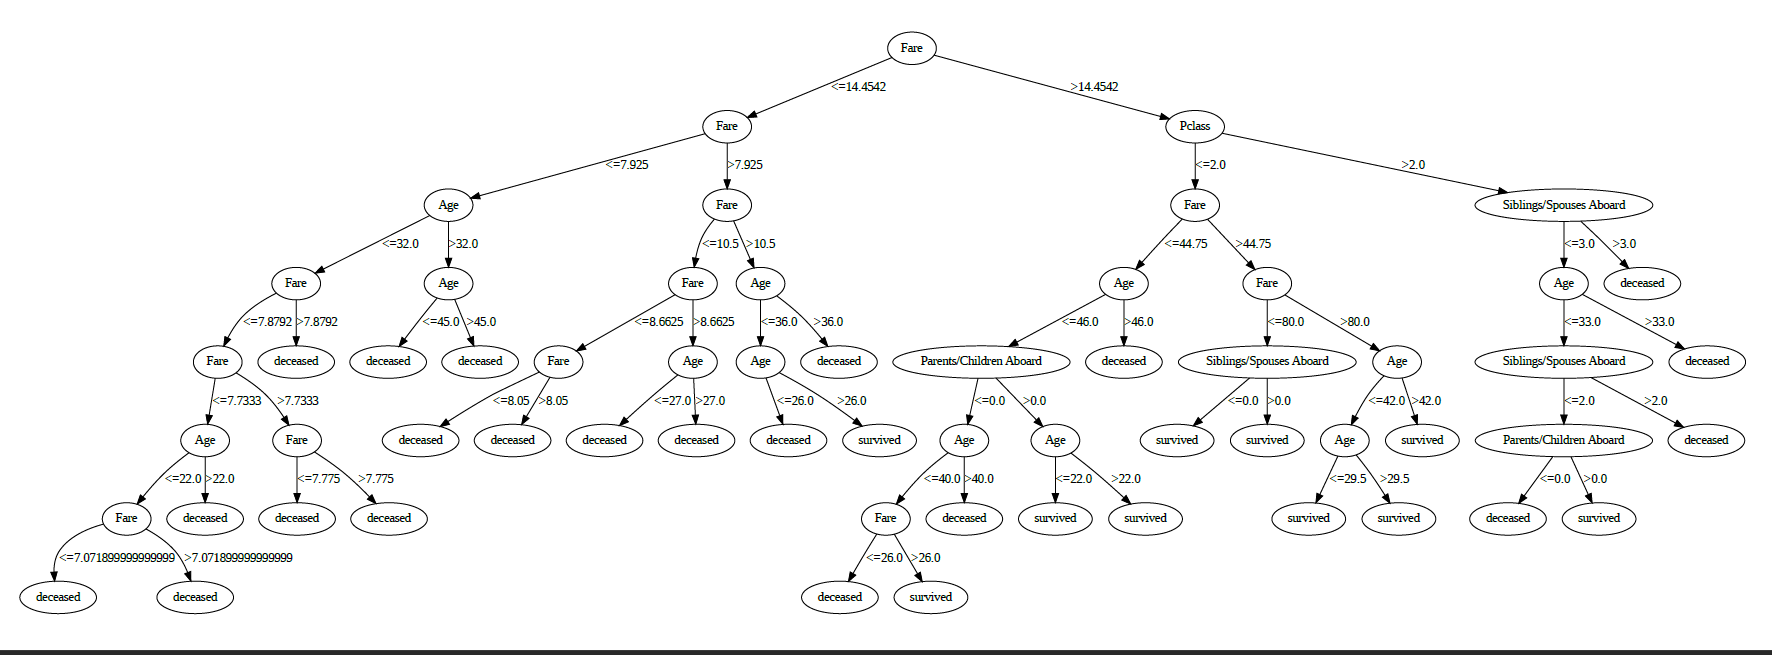
\includegraphics[width=1\textwidth]{rf-feature-dropout/rf_leave_out2.png}}
    \caption{Random Forest excluding feature Sex}
\end{figure}
\begin{figure}
    \ffigbox{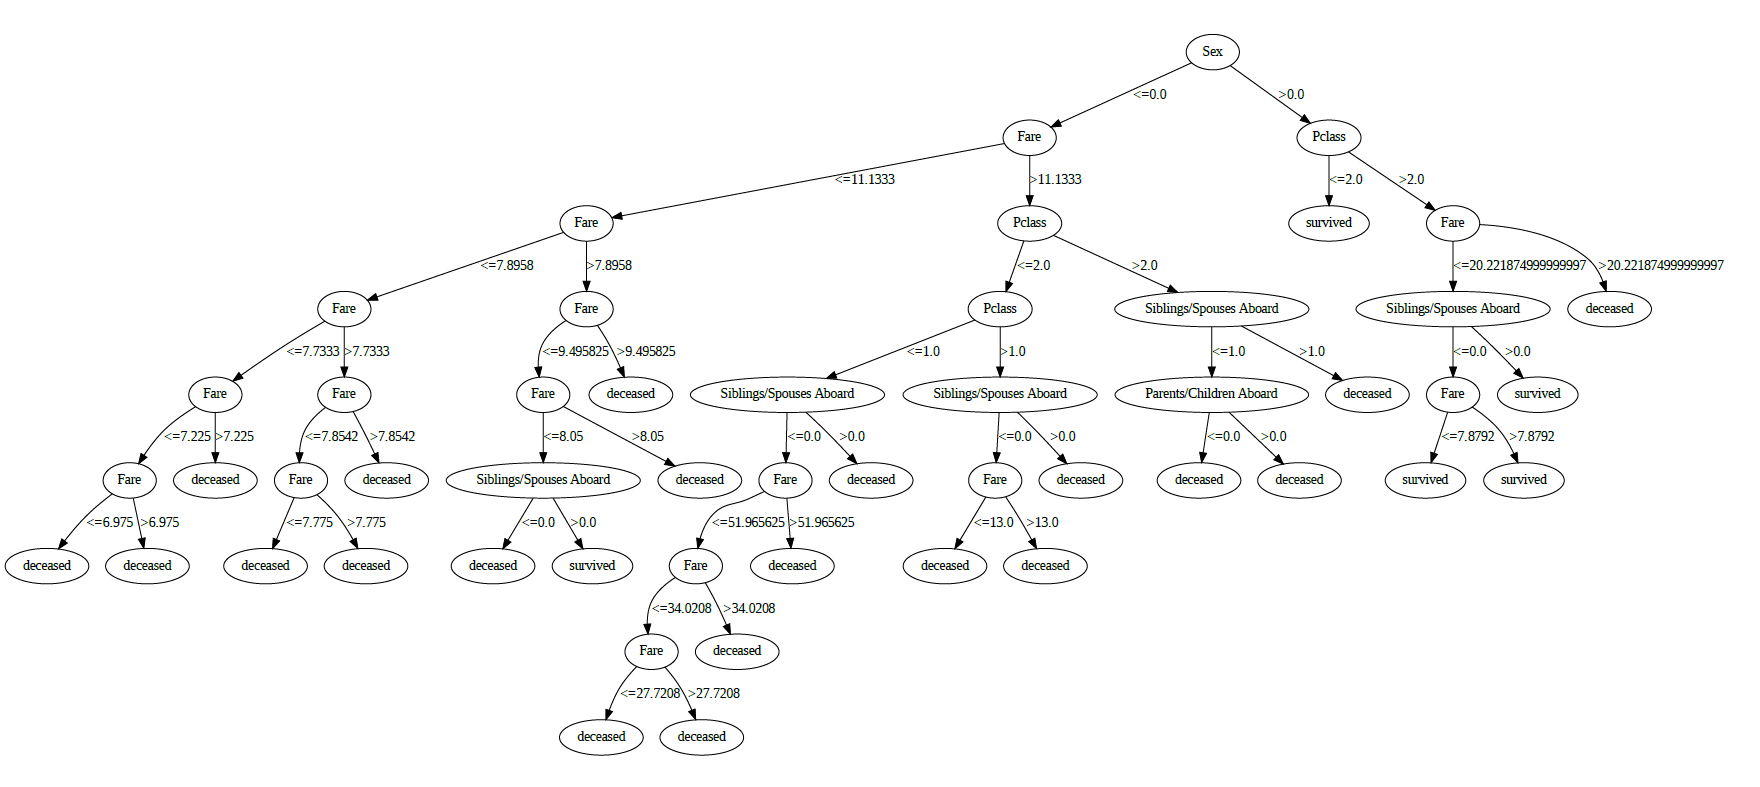
\includegraphics[width=1\textwidth]{rf-feature-dropout/rf_leave_out3.png}}
    \caption{Random Forest excluding feature Age}
\end{figure}
\begin{figure}
    \ffigbox{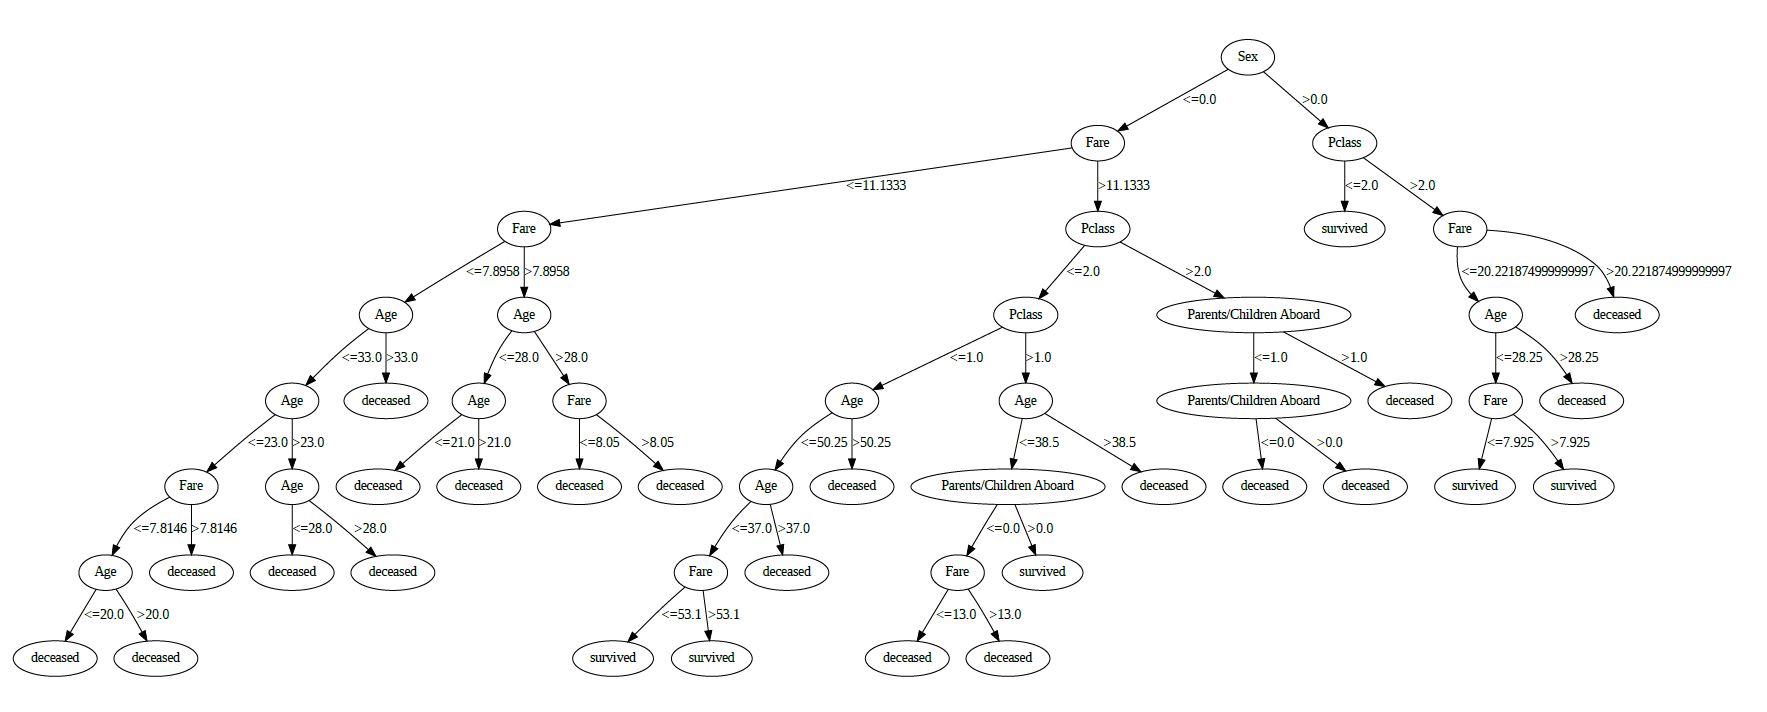
\includegraphics[width=1\textwidth]{rf-feature-dropout/rf_leave_out4.png}}
    \caption{Random Forest excluding feature Siblings/Spouses Aboard}
\end{figure}
\begin{figure}
    \ffigbox{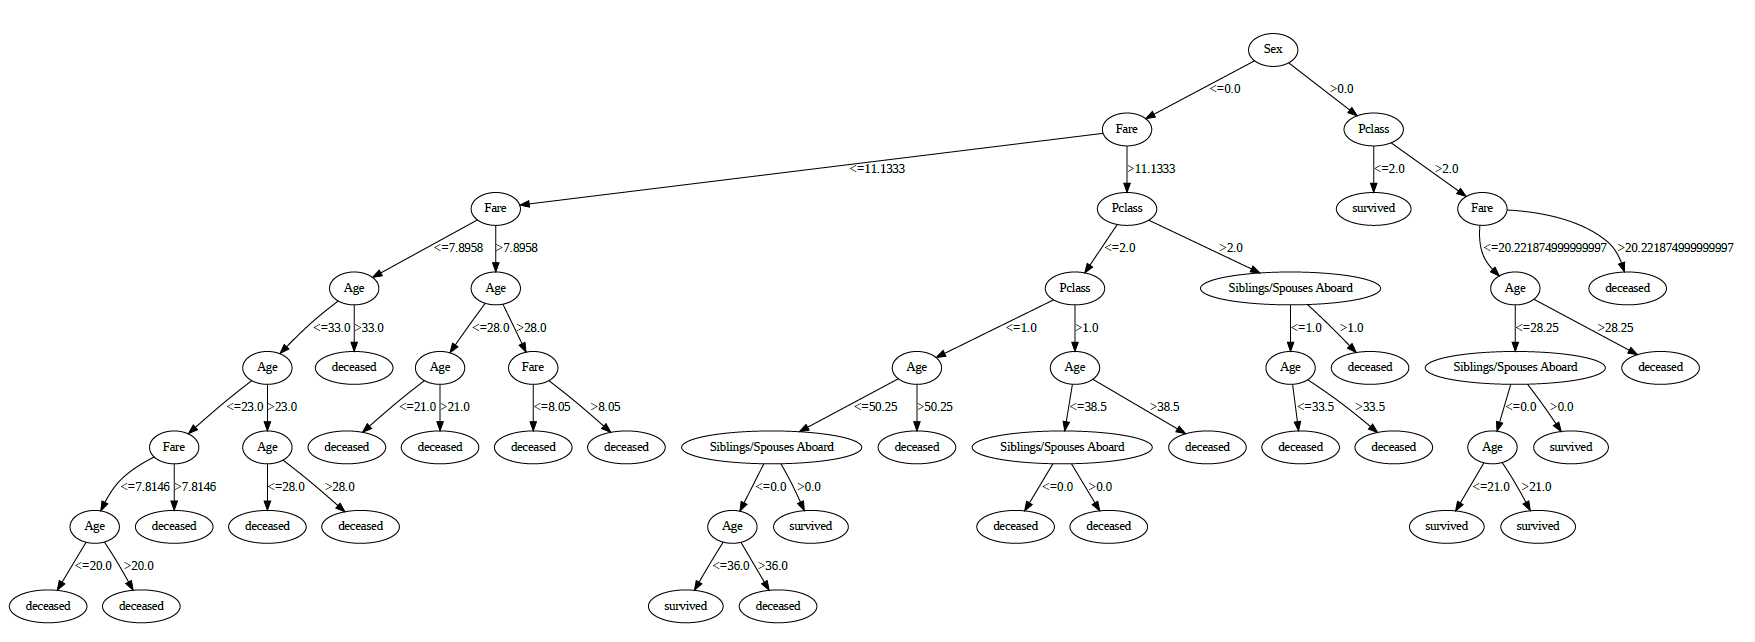
\includegraphics[width=1\textwidth]{rf-feature-dropout/rf_leave_out5.png}}
    \caption{Random Forest excluding feature Parents/Children Aboard}
\end{figure}
\begin{figure}
    \ffigbox{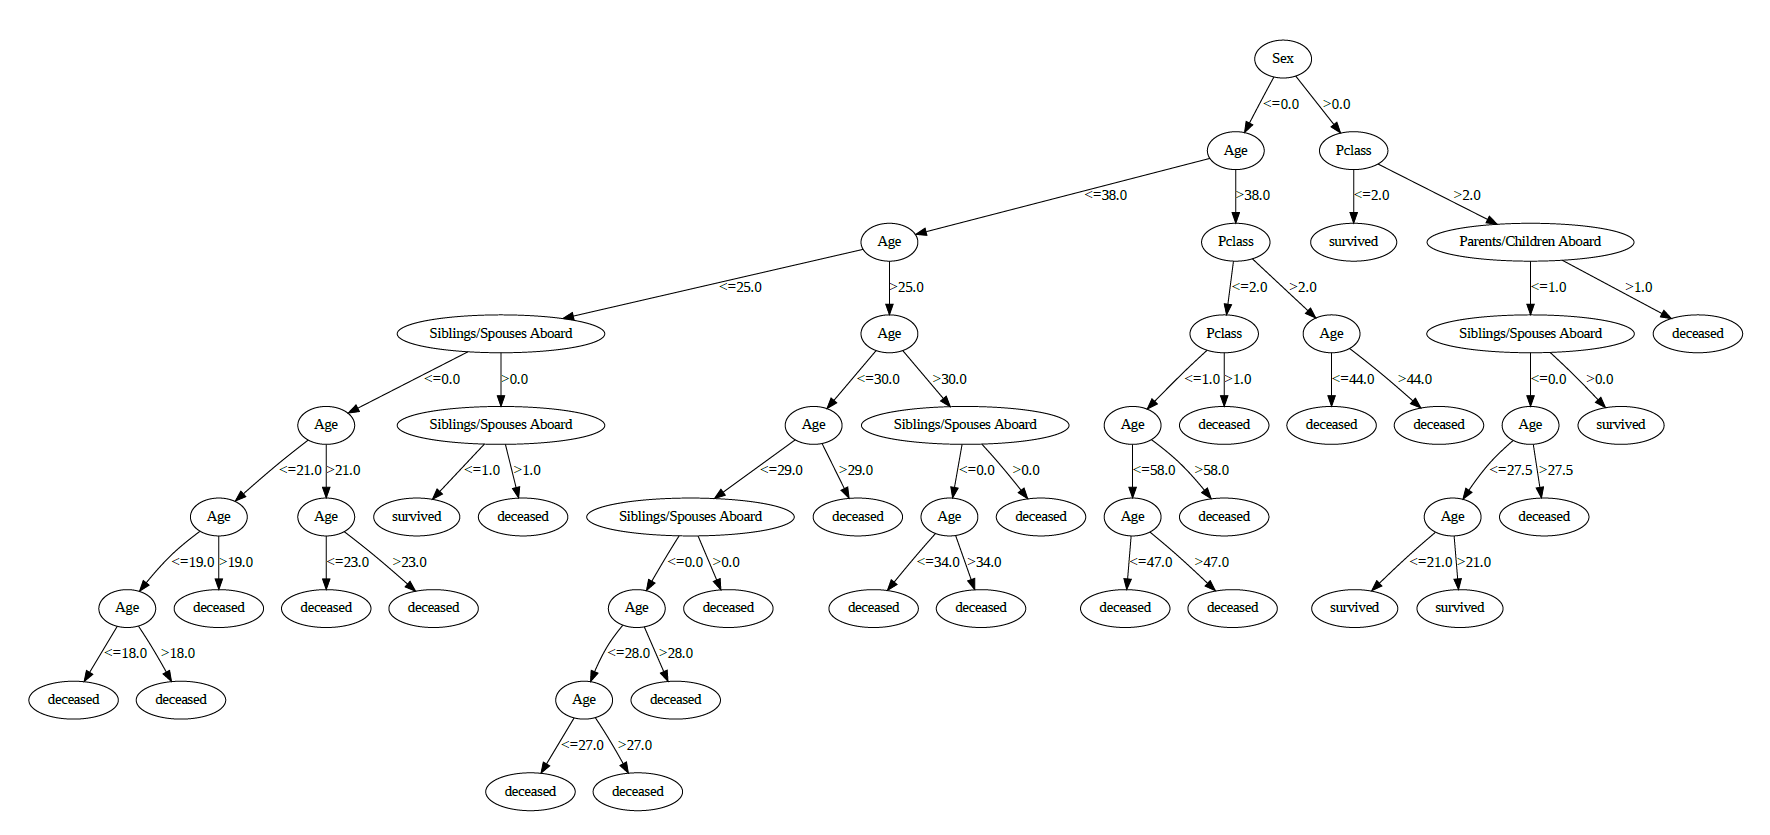
\includegraphics[width=1\textwidth]{rf-feature-dropout/rf_leave_out6.png}}
    \caption{Random Forest excluding feature Fare}
\end{figure}
\subsection{b}
Accuracy obtained by leave out method is 80\%
\subsection{c}
Applying this model to the own feature we get [[1], [0], [0], [0], [0], [0]].
So, it shows we wont survive which is inline with decision tree.
\section{9}
Yes, all the models random forest with leave out, random sampling, decision Tree and logistic regression predicted 0 for my feature vector. 
Logistic regression is the simplest model and easy to use and it is not effected by  as we can stop after few iterations and its easy to tune. We can also get the confidence interval for the predictions. Its easy to store and export the model  as we have just an array of parameters.
On the other hand decision trees and random forest provide intuitive graph representation of decision taken at each step. So, we get the advantage of explainability. Decision tress might be effected by the overfitting and bias where cross validation helps in minimizing this as we test across different batches and random sampling. So, I would like to use random forest with cross validation.
The observed accuracies are: \\
\\
\begin{center}
    \begin{tabular}{|c|c|} 
\hline
Model & Accuracy(\%)\\
\hline % Top horizontal line
Logistic Regression & 80\\ % Row separator (\\)
\hline % Bottom horizontal line
Decision Tree with cross-validation& 79.54\\
\hline
Random Forest with sampling& 79.1\\
\hline
Random Forest with feature dropout& 80\\
\hline
\end{tabular}
\end{center}
\section{10}
\begin{align*}
    I(X;Y) &= \sum_{x \in \mathcal{X}, y \in \mathcal{Y}} P(x,y) \log \frac{P(x,y)}{P(x)P(y)} \\
&= \sum_{x \in \mathcal{X}, y \in \mathcal{Y}} P(x,y) \log \frac{P(x,y)}{P(x)} - \sum_{x \in \mathcal{X}, y \in \mathcal{Y}} P(x,y) \log P(y) \\
&= \sum_{x \in \mathcal{X}, y \in \mathcal{Y}} P(x)P(y|x) \log P(y|x) - \sum_{x \in \mathcal{X}, y \in \mathcal{Y}} P(x,y) \log P(y) \\
&= \sum_{x \in \mathcal{X}} P(x) \left( \sum_{y \in \mathcal{Y}} P(y|x) \log P(y|x) \right) - \sum_{y \in \mathcal{Y}} P(y) \log P(y) \\
&= - \sum_{x \in \mathcal{X}} P(x) H(Y | X = x) - \sum_{y \in \mathcal{Y}} P(y) \log P(y) \\
&= - H(Y | X) + H(Y) \\
&= H(Y) - H(Y|X) \\
&= I(Y;X)
\end{align*}
\section{Appendix}
Accuracy by 90:10 split is around 80\%. \\
\begin{lstlisting}
import pandas as pd
import numpy as np
import matplotlib.pyplot as plt
import math

df = pd.read_csv('titanic_data.csv')
features  = df.iloc[:,1:].columns.values

split_ratio = 0.9
num_rows = int(split_ratio*len(df))
X_train, X_test = df.iloc[:num_rows,1:].to_numpy(), df.iloc[num_rows:,1:].to_numpy()
Y_train, Y_test = df.iloc[:num_rows,:1].to_numpy(), df.iloc[num_rows:,:1].to_numpy()

percentiles = np.linspace(0, 100, 3 + 2)[1:-1]
X = np.array([1,2,3,54,22,2,1,34,54,26])
quantiles = np.percentile(X, percentiles)

#section 4.2, 4.3
class DecisionTree:

  def __init__(self, num_of_splits_per_feature):
      self.num_of_splits_per_feature = num_of_splits_per_feature
      self.num_of_samples = 0
      self.root = None

  def fit_training_data(self, X_train, Y_train):
    self.num_of_samples = len(Y_train)
    # self.Y_train = Y_train
    self.root = self.build_tree(X_train, Y_train)
  
  def build_tree(self, X_data, Y_data):
    subsample_size = len(Y_data)
    #verify if the sample is less than 5% of whole data
    #if yes exit as leaf node
    if subsample_size <= int(0.05*self.num_of_samples):
      # print('current path ends as the sample space is less than 5% of total sample size')
      node = TreeNode(None, None)
      node.isLeaf = True
      if np.sum(Y_data) >= subsample_size//2:
        node.Y_pred = 1
      return node

    #find the feature with max mutual information  
    max_gain = 0
    feature_column, threshold  = 0 , 0
    for i in range(X_data.shape[1]):
      #if the feature is continous compare quartiles 
      percentiles = np.linspace(0, 100, self.num_of_splits_per_feature + 2)[1:-1]
      quantiles = set(np.percentile(X_data[:, i], percentiles))
      for quantile in quantiles:
        curr_gain = self.mutual_information(self.normalize_data(X_data[:, i], quantile), Y_data)
        if curr_gain > max_gain:
          feature_column, threshold, max_gain = i, quantile, curr_gain
    
    #if the resulting gain is small we can end as leaf node
    if max_gain <= 0.05:
      node = TreeNode(None, None)
      node.isLeaf = True
      if np.sum(Y_data) >= subsample_size//2:
        node.Y_pred = 1
      return node

    #split the data accourding to max gain feature 
    # Create a boolean mask based on the feature value
    zipped_data = np.hstack((X_data, Y_data.reshape([-1,1])))
    mask = X_data[:, feature_column] <= threshold 
    # Split the data into two parts
    left_data = zipped_data[mask]
    right_data = zipped_data[~mask]

    node = TreeNode(feature_column=feature_column, threshold=threshold)
    node.left = self.build_tree(left_data[:, :-1], left_data[:, -1])
    node.right = self.build_tree(right_data[:, :-1], right_data[:, -1])
    return node
  
  def normalize_data(self, X, threshold):
    return [1 if X[i] <= threshold else 0 for i in range(len(X))]

  #4.2
  def mutual_information(self, X_data, Y_data):
    subsample_size = len(Y_data)
    p_x_1 = np.sum(X_data)/subsample_size
    entropy_x = self.entropy_helper(p_x_1) + self.entropy_helper(1-p_x_1)

    #conditional entropy 
    count_x_1_y_1, count_x_0_y_1, count_x_0_y_0, count_x_1_y_0 = 0,0,0,0
    for i in range(subsample_size):
      if X_data[i] == 1 and Y_data[i] == 1:
        count_x_1_y_1 += 1
      elif X_data[i] == 0 and Y_data[i] == 1:
        count_x_0_y_1 += 1
      elif  X_data[i] == 0 and Y_data[i] == 0:
        count_x_0_y_0 == 1
      else:
        count_x_1_y_0 += 1
    
    count_y_1 = np.sum(Y_data)
    count_y_0 = len(Y_data) - count_y_1
    entropy_x_given_y = ((count_y_1*self.entropy_helper(count_x_1_y_1/count_y_1) \
                      + count_y_1*self.entropy_helper(count_x_0_y_1/count_y_1)) if count_y_1 != 0 else 0 )\
                      + (count_y_0*self.entropy_helper(count_x_0_y_0/count_y_0) \
                      + count_y_0*self.entropy_helper(count_x_1_y_0/count_y_0)) if count_y_0 != 0 else 0

    entropy_x_given_y /= subsample_size
    #info gain 
    return entropy_x - entropy_x_given_y

  def entropy_helper(self,prob):
    if prob == 0:
      return 0
    return prob*math.log2(1/prob)
    
class TreeNode:

  def __init__(self, feature_column, threshold):
    self.feature_column = feature_column
    self.threshold = threshold
    self.left = None
    self.right = None
    self.isLeaf = False
    self.Y_pred = 0
import graphviz as gv

# Define a graph object
class VisualizeGraph:
  def __init__(self, root, features):
    self.node_index = 1
    self.graph = gv.Digraph()
    self.graph.node(str(self.node_index), features[root.feature_column])
    self.node_index += 1
    self.features = features
    self.build_graph(root, 1)


# Add nodes
  def build_graph(self,node, parent_index):
    #left node 
    if node.left.isLeaf: 
      value = 'survived' if node.left.Y_pred == 1 else 'deceased'
      self.graph.node(str(self.node_index), value)
      self.graph.edge(str(parent_index), str(self.node_index), label=f'<={node.threshold}')
      self.node_index += 1
    else:
      self.graph.node(str(self.node_index), label = self.features[node.left.feature_column])
      self.graph.edge( str(parent_index), str(self.node_index), label=f'<={node.threshold}')
      self.node_index += 1
      self.build_graph(node.left, self.node_index-1)


    #right node
    if node.right.isLeaf: 
      value = 'survived' if node.right.Y_pred == 1 else 'deceased'
      self.graph.node(str(self.node_index), value)
      self.graph.edge(str(parent_index), str(self.node_index), label=f'>{node.threshold}')
      self.node_index += 1
    else:
      self.graph.node(str(self.node_index), label = self.features[node.right.feature_column])
      self.graph.edge(str(parent_index), str(self.node_index), label=f'>{node.threshold}')
      self.node_index += 1
      self.build_graph(node.right, self.node_index-1)

#############################################
#section 4.5 
#10 fold cross validation for decision tree
folds = 10
validation_ratio = folds/100
num_samples = len(df)
test_block_size = int(num_samples*validation_ratio)

accuracy = np.zeros(folds)
#for each fold find the accuracy
for i in range(folds):
  mask = df.index.isin(range(i*test_block_size, (i+1)*test_block_size))
  train_data, test_data = df.iloc[~mask, :].to_numpy(), df.iloc[mask, :].to_numpy()
  X_train, Y_train = train_data[:, 1:], train_data[:, :1]
  X_test, Y_test = test_data[:, 1:], test_data[:, :1]

  #build decision tree
  tree = DecisionTree(3)
  tree.fit_training_data(X_train, Y_train)

  #predict and find accuracy
  accuracy[i] = test(tree, X_test, Y_test)

mean_accuracy = np.mean(accuracy)
print(mean_accuracy)
##############################################
#section 4.6
X_new = np.array([2,
    0,
    25,
    0,
    0,
    20]).reshape([6,1])
node = decisionTree.root
while not node.isLeaf:
  if X_new[node.feature_column] <= node.threshold:
    node = node.left
  else:
    node = node.right
print(node.Y_pred)
#################################################
#section 4.7 a
#section 4.7 a 
#random forest 
def random_forest(df):

  descision_trees = []
  for i in range(5):
    #random sampling 80% of dataset
    df1 = df.sample(frac=0.8)
    X_rf_1,Y_rf_1 = df1.iloc[:,1:].to_numpy(), df1.iloc[:,0].to_numpy()

    #build decision tree
    decisionTree = DecisionTree(3)
    decisionTree.fit_training_data(X_rf_1, Y_rf_1)

    descision_trees.append(decisionTree)
    #save the decision tree as image
    # vg_graph = VisualizeGraph(decisionTree.root, features)
    # vg_graph.graph.render(f"graph_rf{i+1}.png")
  return descision_trees

random_forest(df)

#section 4.7 b
#section 4.7 b
#10 fold cross validation for decision tree

def predict(decisionTree, X_test):
  y_pred = []
  for i in range(X_test.shape[0]):
    node = decisionTree.root
    while not node.isLeaf:
      if X_test[i, node.feature_column] <= node.threshold:
        node = node.left
      else:
        node = node.right
    
    y_pred.append(node.Y_pred)
    
  #apredictions
  return np.array(y_pred)
  
folds = 10
validation_ratio = folds/100
num_samples = len(df)
test_block_size = int(num_samples*validation_ratio)

accuracy = np.zeros(folds)
#for each fold find the accuracy
for i in range(folds):
  mask = df.index.isin(range(i*test_block_size, (i+1)*test_block_size))
  train_data, test_data = df.iloc[~mask, :].to_numpy(), df.iloc[mask, :].to_numpy()
  X_train, Y_train = train_data[:, 1:], train_data[:, :1]
  X_test, Y_test = test_data[:, 1:], test_data[:, :1]

  #build random forests 
  trees = random_forest(df.iloc[~mask, :])
  y_pred = np.zeros(test_block_size)

  for tree in trees:
    y_pred += predict(tree, X_test)

  pred_threshold = (1+len(trees))//2

  y_pred_cummulative = [1 if y_pred[i] >= pred_threshold else 0 for i in range(test_block_size)]
  #find accuracy
  correct_predictions = 0
  for j in range(test_block_size):
    if y_pred_cummulative[j] == Y_test[j]:
      correct_predictions += 1
  accuracy[i] = correct_predictions/test_block_size

mean_accuracy = np.mean(accuracy)
print(mean_accuracy)
###############################################
#section 4.7 c
for tree in trees:
  print(predict(tree, X_new.reshape([1,-1])))
ouput : [[0],[0],[0],[0],[0]]
##############################################
#section 4.8 a
#random forest with excluding feature
def random_forest_with_leave_out(df):

  descision_trees = []
  for i in range(6):
    #dropping feature using feature map which containes features to index map
    df1 = df.drop(columns=features[i])
    feature_map = np.delete(features, i)
    X_rf_1,Y_rf_1 = df1.iloc[:,1:].to_numpy(), df1.iloc[:,0].to_numpy()

    #build decision tree
    decisionTree = DecisionTree(3)
    decisionTree.fit_training_data(X_rf_1, Y_rf_1)

    descision_trees.append(decisionTree)
    #save the decision tree as image
    # vg_graph = VisualizeGraph(decisionTree.root, feature_map)
    # vg_graph.graph.render(f"graph_rf_leave_out{i+1}.png")
  return descision_trees

random_forest_with_leave_out(df)
####################################################
#section 4.8 b
#section 4.8 b 
  
folds = 10
validation_ratio = folds/100
num_samples = len(df)
test_block_size = int(num_samples*validation_ratio)

accuracy = np.zeros(folds)
#for each fold find the accuracy
for i in range(folds):
  mask = df.index.isin(range(i*test_block_size, (i+1)*test_block_size))
  train_data, test_data = df.iloc[~mask, :].to_numpy(), df.iloc[mask, :].to_numpy()
  X_train, Y_train = train_data[:, 1:], train_data[:, :1]
  X_test, Y_test = test_data[:, 1:], test_data[:, :1]

  #build random forests 
  trees = random_forest_with_leave_out(df.iloc[~mask, :])
  y_pred = np.zeros(test_block_size)

  for index,tree in enumerate(trees):
    #delete the column with index 
    X_data_sliced = np.delete(X_test, index, axis=1)
    y_pred += predict(tree, X_data_sliced)

  pred_threshold = (1+len(trees))//2

  y_pred_cummulative = [1 if y_pred[i] >= pred_threshold else 0 for i in range(test_block_size)]
  #find accuracy
  correct_predictions = 0
  for j in range(test_block_size):
    if y_pred_cummulative[j] == Y_test[j]:
      correct_predictions += 1
  accuracy[i] = correct_predictions/test_block_size

mean_accuracy = np.mean(accuracy)
print(mean_accuracy)
#######################################################
#section 4.8 c
for tree in trees:
  print(predict(tree, X_new.reshape([1,-1])))
\end{lstlisting}
\end{document}
